\documentclass[landscape]{seminar}

\usepackage{color}
\definecolor{darkblue}{rgb}{.0, .0, .6} 

\usepackage[dvips]{graphicx}

\usepackage{hyperref}
\hypersetup{
  pdfmenubar=true,
  pdftoolbar=true,
  pdfpagemode={None}
}

\pagestyle{empty}

\renewcommand{\printlandscape}{\special{landscape}}

\begin{document}

%%%%%%%%%%%%%%%%%%%%%%%%%%%%%%%%%%%%%%%%%%%%%%%%%%%%%%%%%%%%%%%%%%%%%%%%%%%%%%%%
\begin{slide}

\begin{center}
{\color{darkblue} \large Vertical Frontal Circulations for Variations in Tropopause Height \\ \rule[0.15in]{\textwidth}{.03in}}
\end{center}

{\color{darkblue} \large Outline}
\begin{itemize}
\item The Sawyer-Eliassen Equation

\item Vertical Flow for a Sloping Tropopause

\item Vertical Flow with Tropopause Curvature

\item Frontal Interaction with Upper-Level Jet Streak

\item Concluding Remarks
\end{itemize}

\end{slide}
%%%%%%%%%%%%%%%%%%%%%%%%%%%%%%%%%%%%%%%%%%%%%%%%%%%%%%%%%%%%%%%%%%%%%%%%%%%%%%%%
\begin{slide}

\begin{center}
{\color{darkblue} \large The Sawyer-Eliassen Equation \\ \rule[0.15in]{\textwidth}{.03in}}
\end{center}

\begin{itemize}
\item We wish to determine the structure of cross-front vertical flow

\item Assumptions:

\begin{itemize}
  \item Flow is either QG or SG
  \item Flow is symmetric along-front (e.g. in $y$-direction)
\end{itemize}

\item Streamfunction $\psi$ for nongeostrophic flow $(u_{ag},w)$ satisfies the Sawyer-Eliassen (SE) equation(s)

\item The analysis here closely follows Hakim and Keyser (2001)

\end{itemize}

\end{slide}
%%%%%%%%%%%%%%%%%%%%%%%%%%%%%%%%%%%%%%%%%%%%%%%%%%%%%%%%%%%%%%%%%%%%%%%%%%%%%%%%
\begin{slide}

\begin{itemize}
\item QG: \quad $\! N_{\scriptscriptstyle 0}^2 \psi_{xx} + f^2 \psi_{zz} = -2 Q$

\item SG: \quad $N^2 \psi_{xx} - 2 S^2 \psi_{xz} + F^2 \psi_{zz} = -2 Q$

\vskip 10pt
\begin{itemize}
\item[$\rightarrow$]{\small $N^2 = N_{\scriptscriptstyle 0}^2 + b_z$, $S^2 = f v_{gz} = b_{x}$, $F^2 = f(f+v_{gx})$ \\ ($b$ is the buoyancy)}
\end{itemize}
\vskip 10pt

\item $Q = - f \frac{\partial(u_g,v_g)}{\partial(x,z)} \ + $ diabatic and cross-plane (along-front) momentum sources, e.g. jet streak

\item $Q > 0$ represents a frontogenetic source

\item SE equation determines flow required to maintain thermal wind balance in presence of $Q$
\end{itemize}

\end{slide}
%%%%%%%%%%%%%%%%%%%%%%%%%%%%%%%%%%%%%%%%%%%%%%%%%%%%%%%%%%%%%%%%%%%%%%%%%%%%%%%%
\begin{slide}

\begin{itemize}
\item For QG, rescale $z$ by some height $H$ and $x$ by Rossby radius $L_{QG} = N_{\scriptscriptstyle 0}H/f$

\item $Q$ and $\psi$ are rescaled to be $O(1)$

\item SE equation becomes \fbox{$\psi_{xx} + \psi_{zz} = -2Q$}

\item For SG, change coordinates to $(X,Z) = (x+v_g/f,z)$, and scale in a similar manner

\item SE equation becomes \fbox{$\psi_{XX} + \psi_{ZZ} = -2Q$}

\item Both cases reduce to Poisson's equation, which can be solved in a number of ways
\end{itemize}

\end{slide}
%%%%%%%%%%%%%%%%%%%%%%%%%%%%%%%%%%%%%%%%%%%%%%%%%%%%%%%%%%%%%%%%%%%%%%%%%%%%%%%%
\begin{slide}

\begin{itemize}
\item Assume that sources are highly localized, as if point sources (i.e. $\delta$-functions)

\item For $Q$ at $\mathbf{r_{\scriptscriptstyle 0}}$ we must solve 
$\psi_{xx} + \psi_{yy} = -2 Q_0 \delta(\mathbf{r - r_{\scriptscriptstyle 0}})$

\item This is a Green function problem; solution is $\psi = -\frac{Q_0}{\pi} \log |\mathbf{r - r_{\scriptscriptstyle 0}}|$

\item Flow due to a number of sources is obtained by adding together $\psi$ solutions for each source
\end{itemize}

\end{slide}
%%%%%%%%%%%%%%%%%%%%%%%%%%%%%%%%%%%%%%%%%%%%%%%%%%%%%%%%%%%%%%%%%%%%%%%%%%%%%%%%
\begin{slide}

\begin{center}
{\color{darkblue} \large Vertical Flow for a Sloping Tropopause \\ \rule[0.15in]{\textwidth}{.03in}}

\begin{figure}
\includegraphics[width=1in]{slides_fig.1}
\end{figure}
\end{center}

\begin{itemize}
\item We model sloping effects by considering a wedge-shaped region

\item Assume $\psi=0$ on edges so that $\psi = 0$ everywhere (i.e. no flow) when no sources are present

\item To determine $\psi$ due to a point source, use the \emph{method of images}
\end{itemize}

\end{slide}
%%%%%%%%%%%%%%%%%%%%%%%%%%%%%%%%%%%%%%%%%%%%%%%%%%%%%%%%%%%%%%%%%%%%%%%%%%%%%%%%
\begin{slide}

\begin{center}

{\color{darkblue} The Method of Images}

\begin{figure}
\includegraphics[width=1.8in]{slides_fig.2}
\end{figure}
\end{center}

\begin{itemize}
\item Method relies on uniqueness: Any solution satisfying the boundary conditions is the only solution

\item For a single boundary with a source $Q$ above, it is balanced by a fictitious source $-Q$ directly below, thereby setting $\psi = 0$ along the boundary

\item $\psi$ must behave as if this fictitious source exists
\end{itemize}

\end{slide}
%%%%%%%%%%%%%%%%%%%%%%%%%%%%%%%%%%%%%%%%%%%%%%%%%%%%%%%%%%%%%%%%%%%%%%%%%%%%%%%%
\begin{slide}

\begin{center}
\begin{figure}
\includegraphics[width = 1.5in]{slides_fig.3}
\end{figure}
\end{center}

\begin{itemize}
\item We can extend this to a wedge, if edge angle is $\theta = \frac{2\pi}{n}$ and $n$ is an even integer (In figure, $n$ = 8)

\item Images can't be used for an arbitrary angle, but an analytic solution exists

\item For simplicity, we restrict ourselves to cases supporting images
\end{itemize}

\end{slide}
%%%%%%%%%%%%%%%%%%%%%%%%%%%%%%%%%%%%%%%%%%%%%%%%%%%%%%%%%%%%%%%%%%%%%%%%%%%%%%%%
\begin{slide}

\begin{itemize}
\item This method produces the solution for $\psi$ due to a single source

\item The nondimensional QG solution is
\end{itemize}

\[
\ \ \ \ \psi = -\frac{Q}{\pi} \sum_{k=0}^{\frac{n}{2}-1} \log \! \left[\frac{(x-a \cos(\frac{4 \pi k}{n} + \gamma))^2 + (z-a \sin(\frac{4 \pi k}{n} + \gamma))^2}{(x-a \cos(\frac{4 \pi k}{n} - \gamma))^2 + (z-a \sin(\frac{4 \pi k}{n} - \gamma))^2}\right]
\]

\begin{itemize}
\item For SG, evaluate $v_g$ via Taylor series about source location $(x_i,z_i)$ and use with $F^2 = f(f+v_{gx})$ and $S^2 = f v_{gz}$, obtaining
\[
(X-X_i) = \frac{F^2}{f^2}(x-x_i) + \frac{S^2}{f^2} (z-z_i)
\]

\item This equation, along with $Z-Z_i = z-z_i$, is used on the dimensional form of $\psi$ to determine SG streamfunction

\end{itemize}

\end{slide}
%%%%%%%%%%%%%%%%%%%%%%%%%%%%%%%%%%%%%%%%%%%%%%%%%%%%%%%%%%%%%%%%%%%%%%%%%%%%%%%%
\begin{slide}

\begin{center}
QG Streamfunctions
\begin{figure}
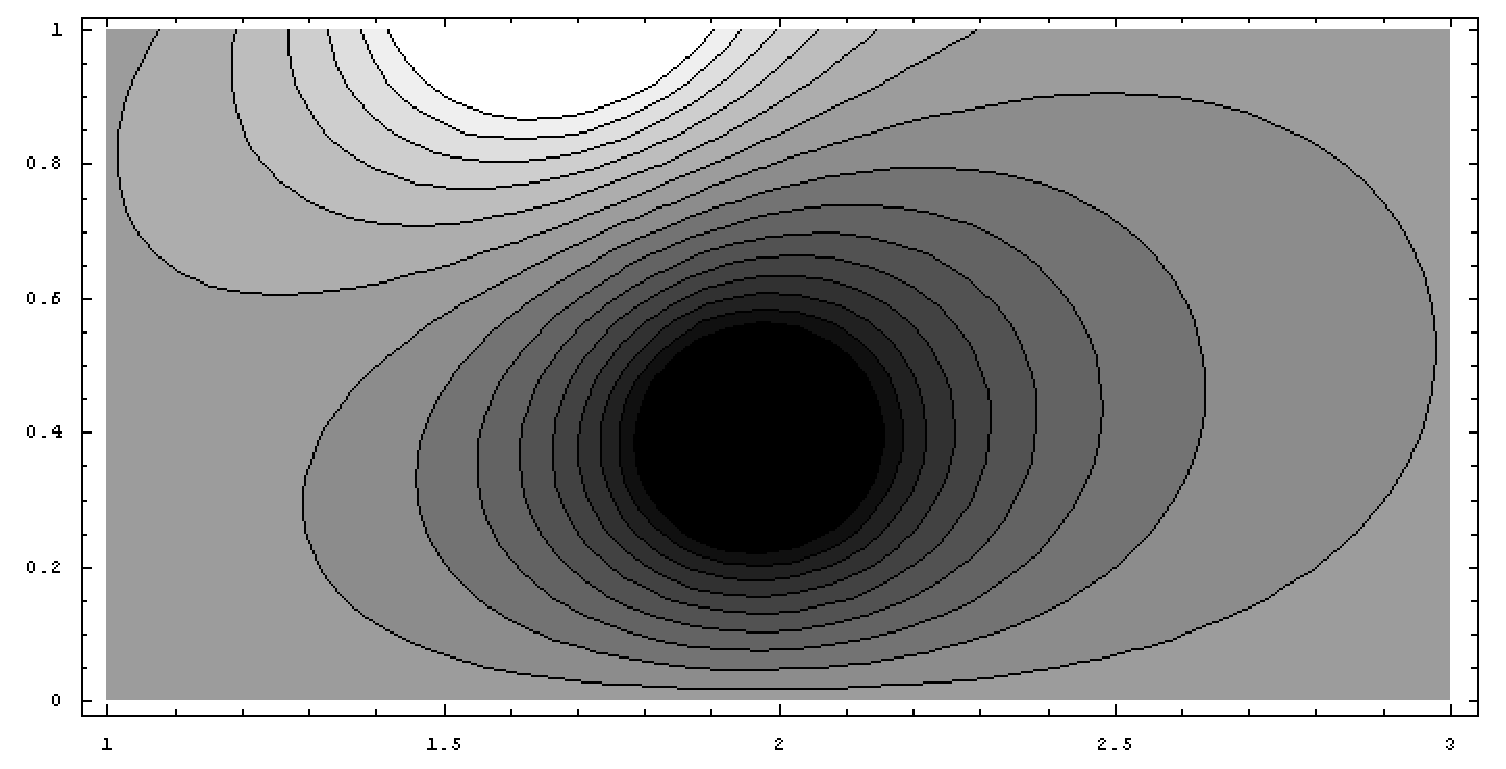
\includegraphics[width=2in]{img/qg_slope_n16_1src_mid.eps}
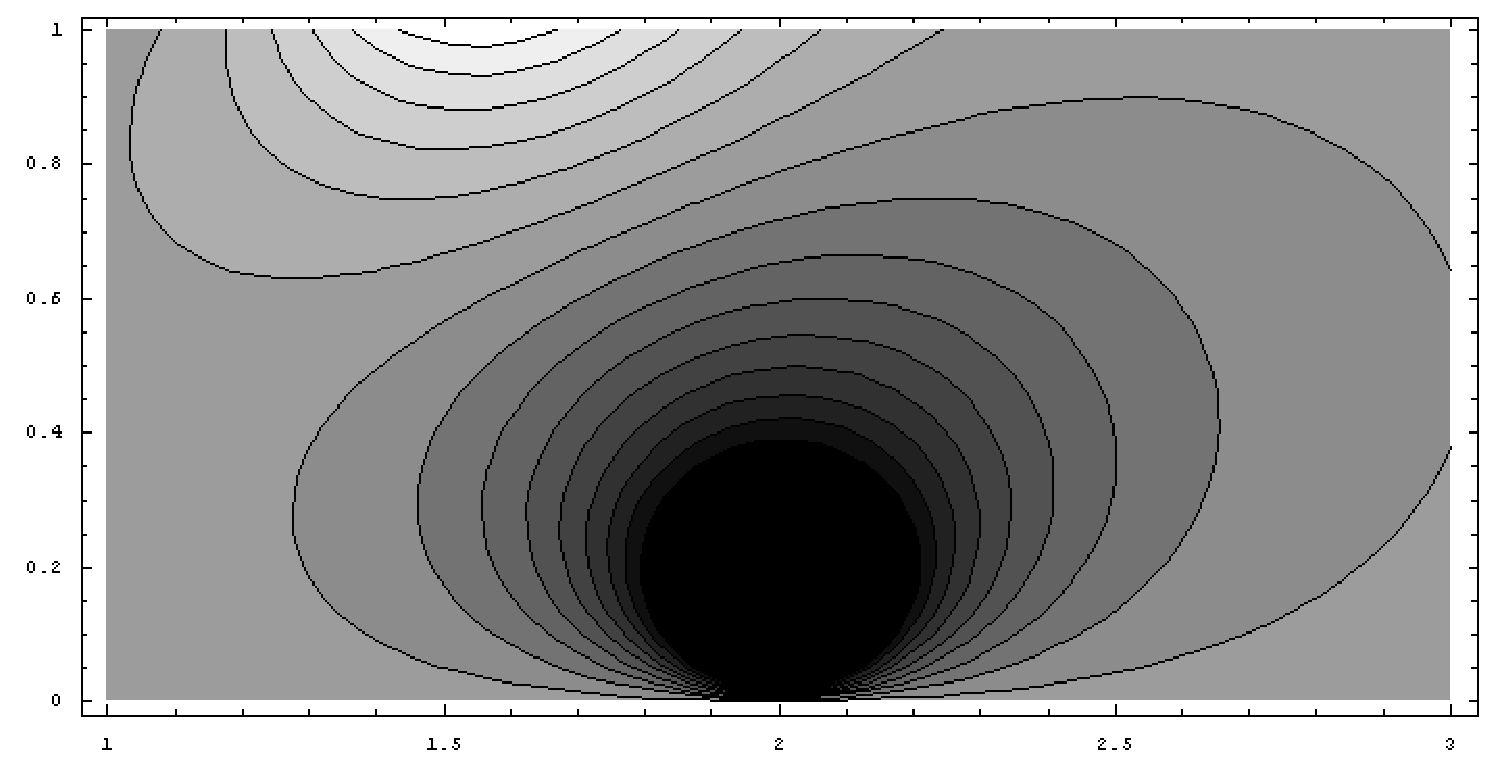
\includegraphics[width=2in]{img/qg_slope_n16_1src_btm.eps}
\title{QG plots}
\end{figure}

SG Streamfunctions
\begin{figure}
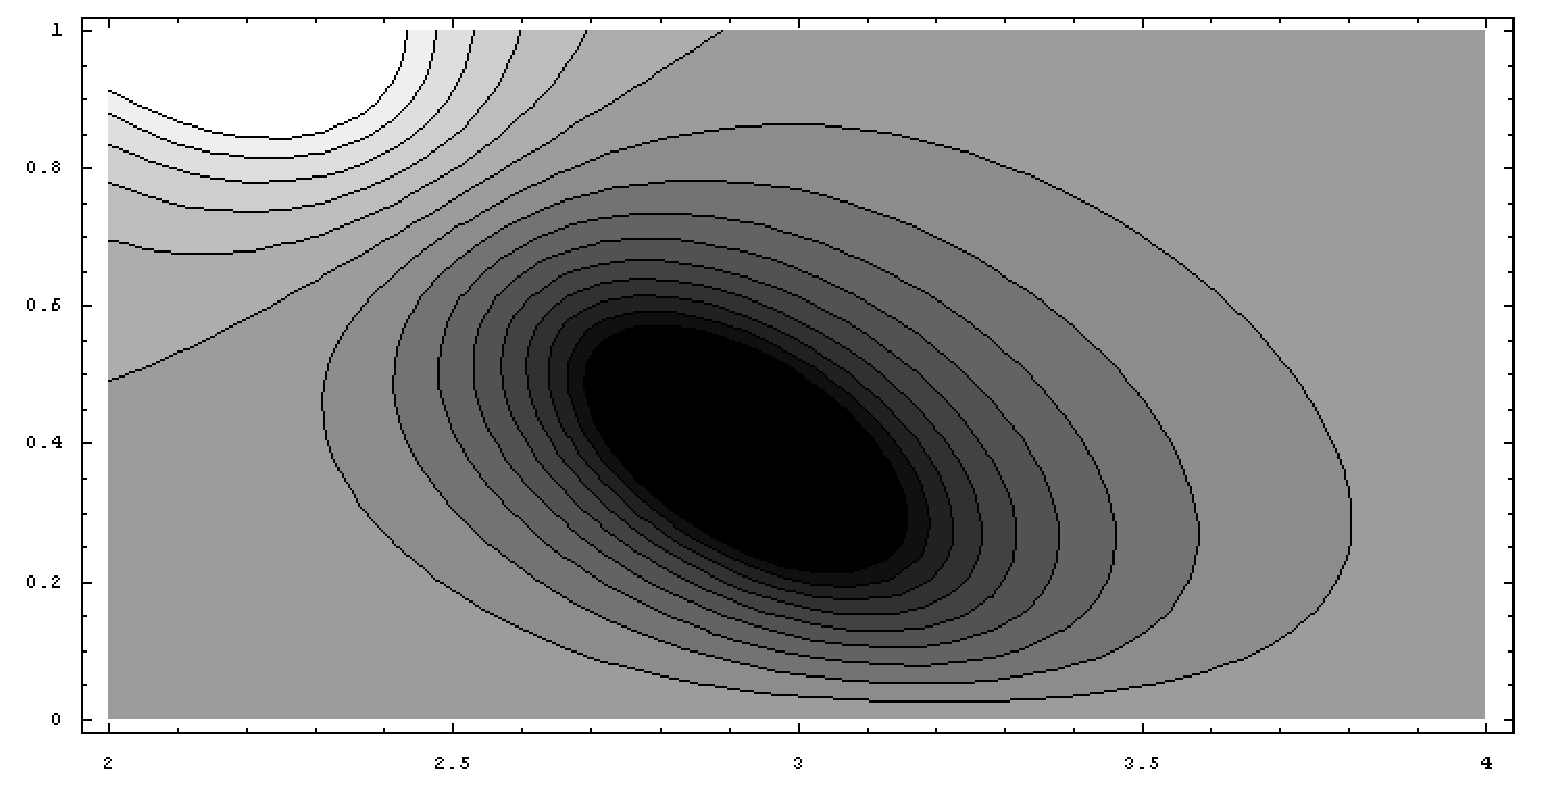
\includegraphics[width=2in]{img/sg_slope_n16_s075_1src_mid.eps}
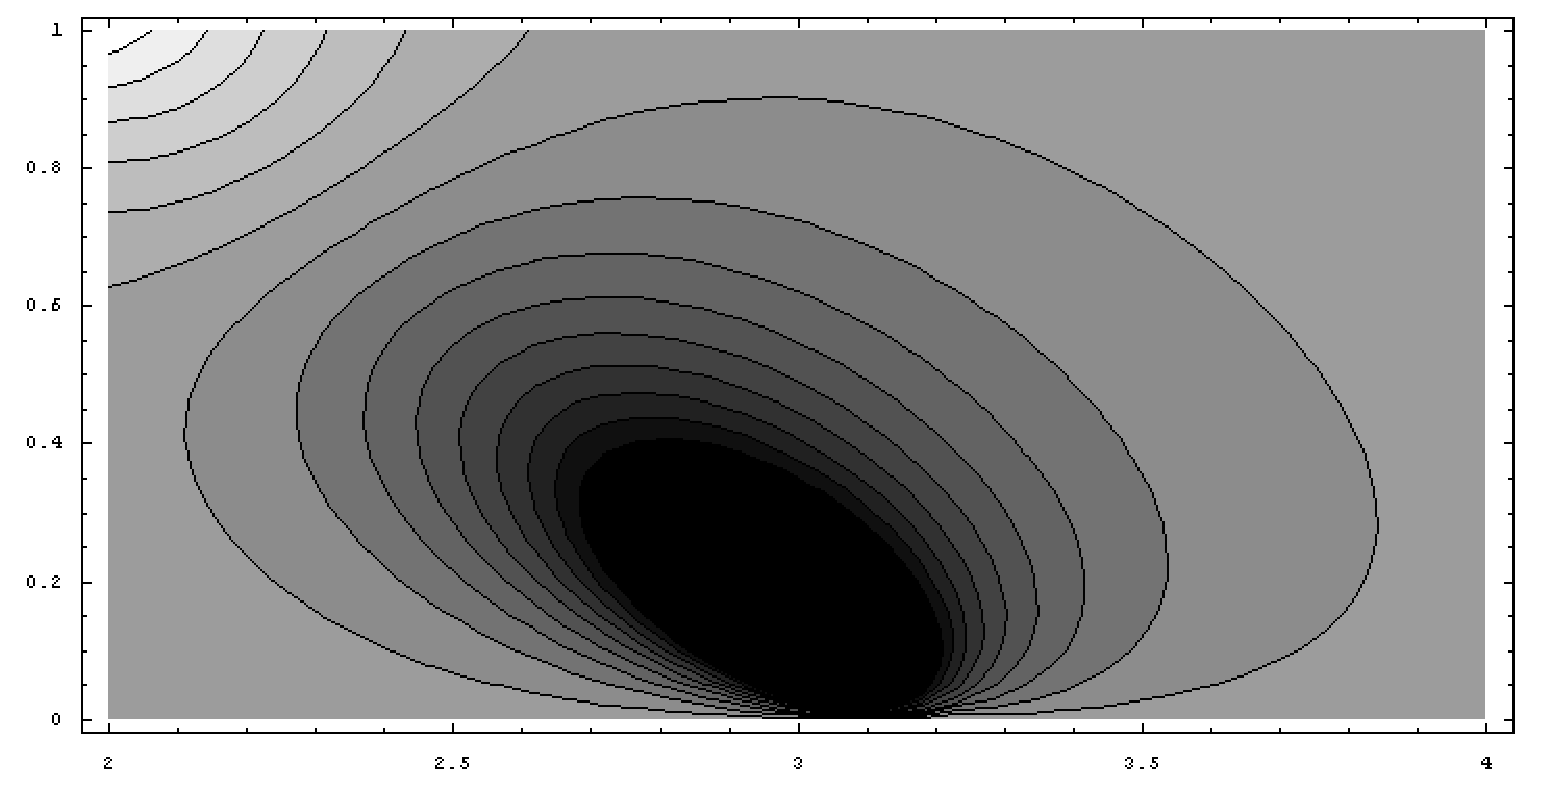
\includegraphics[width=2in]{img/sg_slope_n16_s075_1src_btm.eps}
\end{figure}
\end{center}

\end{slide}
%%%%%%%%%%%%%%%%%%%%%%%%%%%%%%%%%%%%%%%%%%%%%%%%%%%%%%%%%%%%%%%%%%%%%%%%%%%%%%%%
\begin{slide}

\begin{center}
SG Tropopause for Two Sources
\begin{figure}
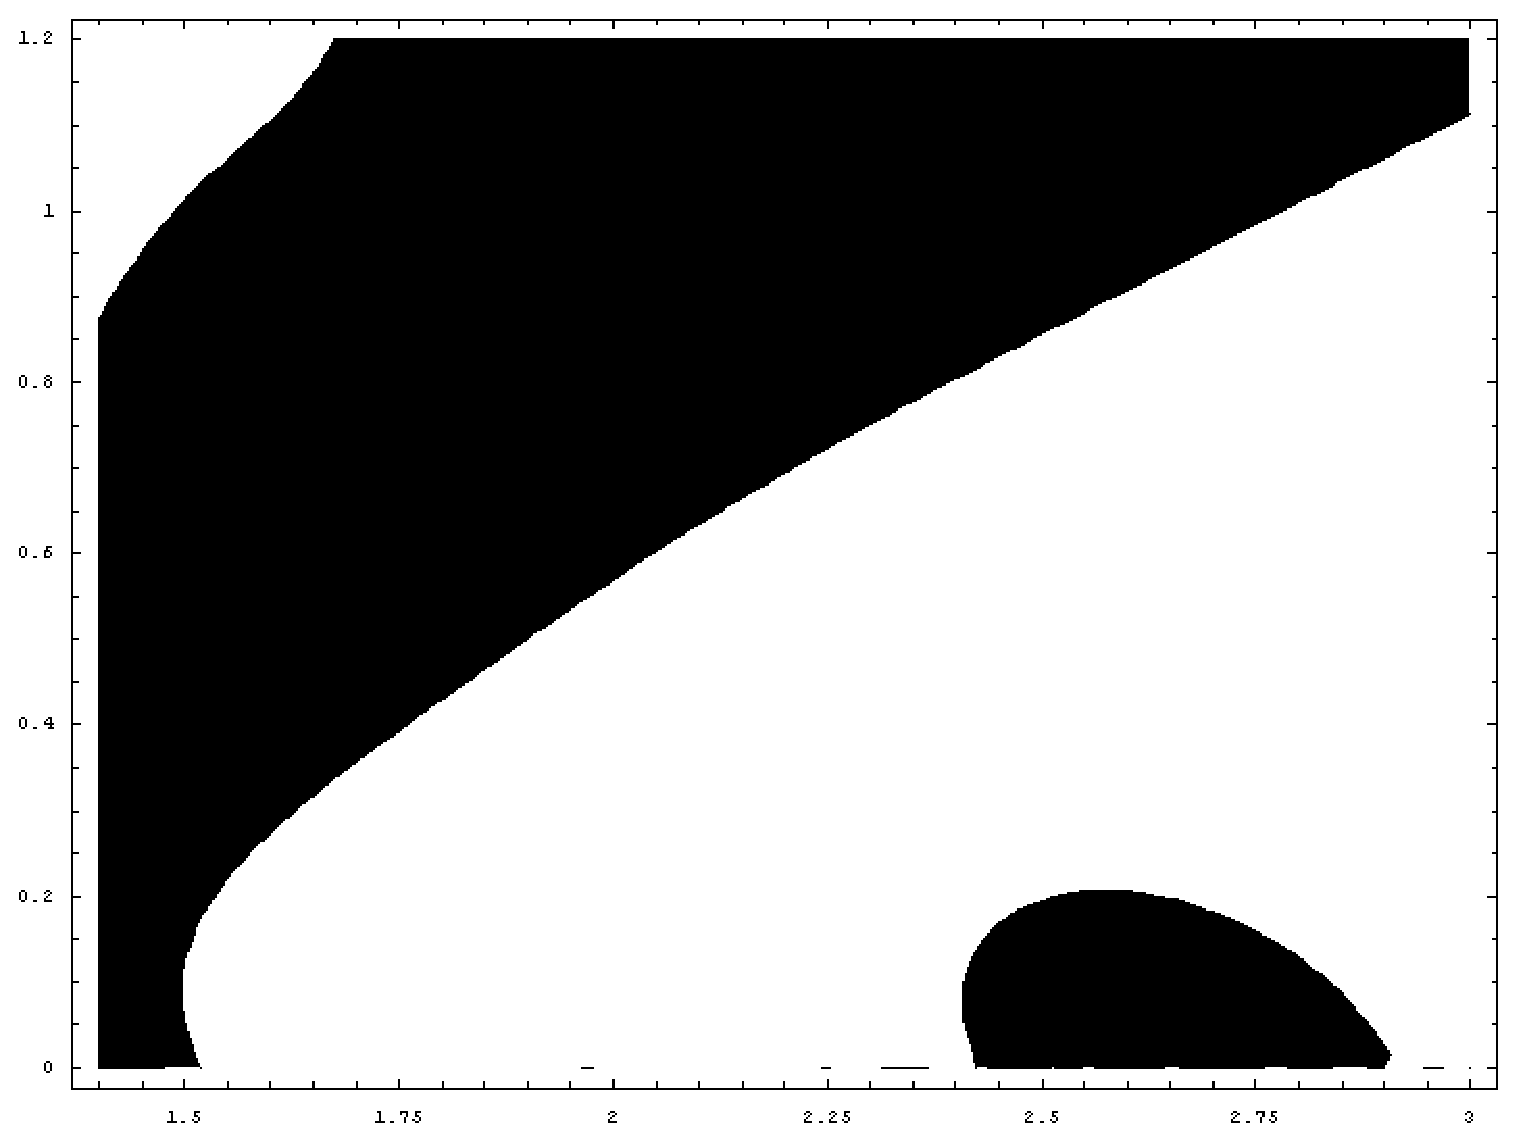
\includegraphics[width=3.5in]{img/sg_slope_2src_surface.eps}
\end{figure}
\end{center}

\end{slide}
%%%%%%%%%%%%%%%%%%%%%%%%%%%%%%%%%%%%%%%%%%%%%%%%%%%%%%%%%%%%%%%%%%%%%%%%%%%%%%%%
\begin{slide}

\begin{center}
{\color{darkblue} \large Vertical Flow with Tropopause Curvature \\ \rule[0.15in]{\textwidth}{.03in}}

\begin{figure}
\includegraphics[width=2in]{slides_fig.4}
\end{figure}
\end{center}

\begin{itemize}
\item Curvature effects are modeled by considering a circular cross-section of radius $a$ that sweeps an angle of $2 \theta_0$
\end{itemize}

\end{slide}
%%%%%%%%%%%%%%%%%%%%%%%%%%%%%%%%%%%%%%%%%%%%%%%%%%%%%%%%%%%%%%%%%%%%%%%%%%%%%%%%
\begin{slide}

\begin{center}
\begin{figure}
\includegraphics[width=2in]{slides_fig.5}
\end{figure}
\end{center}

\begin{itemize}
\item Problem is greatly simplified by changing coordinates

\item Reflect points across a circle of radius $l$, the length of the bottom boundary, by the formula $R = l^2 / r$

\item Based on a \emph{conformal mapping}, so Poisson's equation remains valid

\item Circular arc becomes a wedge, which we have already solved!

\end{itemize}

\end{slide}
%%%%%%%%%%%%%%%%%%%%%%%%%%%%%%%%%%%%%%%%%%%%%%%%%%%%%%%%%%%%%%%%%%%%%%%%%%%%%%%%
\begin{slide}

\begin{center}
QG Streamfunctions
\begin{figure}
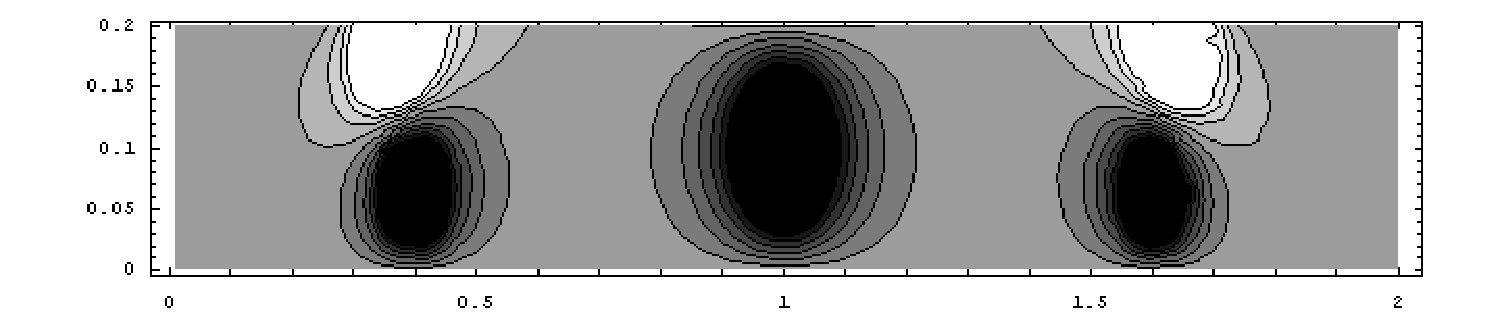
\includegraphics[width=4in]{img/qg_curve_n16_3src_mid.eps}
\end{figure}
\end{center}

\end{slide}
%%%%%%%%%%%%%%%%%%%%%%%%%%%%%%%%%%%%%%%%%%%%%%%%%%%%%%%%%%%%%%%%%%%%%%%%%%%%%%%%
\begin{slide}

\begin{center}
SG Streamfunctions
\begin{figure}
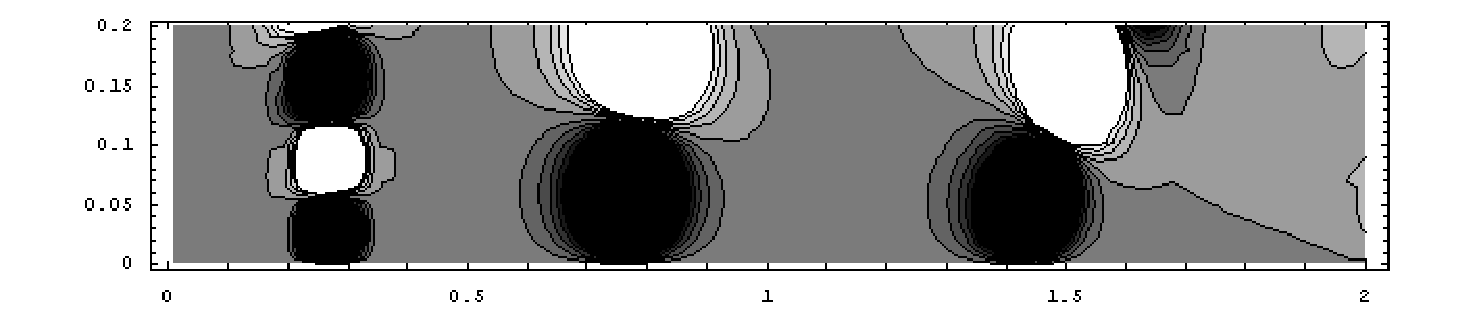
\includegraphics[width=4in]{img/sg_curve_n16_s075_3src_mid.eps}
\end{figure}

SG Tropopause
\begin{figure}
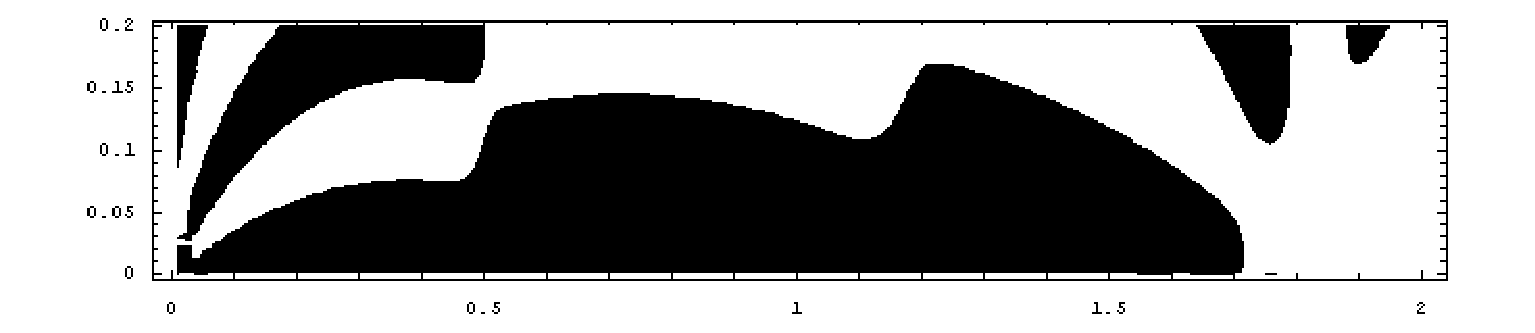
\includegraphics[width=4in]{img/sg_curve_3src_surface.eps}
\end{figure}
\end{center}

\end{slide}
%%%%%%%%%%%%%%%%%%%%%%%%%%%%%%%%%%%%%%%%%%%%%%%%%%%%%%%%%%%%%%%%%%%%%%%%%%%%%%%%
\begin{slide}

\begin{center}
{\color{darkblue} \large Frontal Interaction with Upper-Level Jet Streak \\ \rule[0.15in]{\textwidth}{.03in}}
\end{center}

\begin{itemize}
\item We consider frontal interaction with along-front jet streak, as in Hakim and Keyser

\item Jet streaks are represented by $Q$ anomalies

\item $Q>0$: Jet streak entrance region (accelerations)

\item $Q<0$: Jet streak exit region exit region (deceleration)
\end{itemize}

\end{slide}
%%%%%%%%%%%%%%%%%%%%%%%%%%%%%%%%%%%%%%%%%%%%%%%%%%%%%%%%%%%%%%%%%%%%%%%%%%%%%%%%
\begin{slide}

\begin{center}
Upper-Level Jet Streak Exit Region Directly Atop a Surface Frontal Zone
\begin{figure}
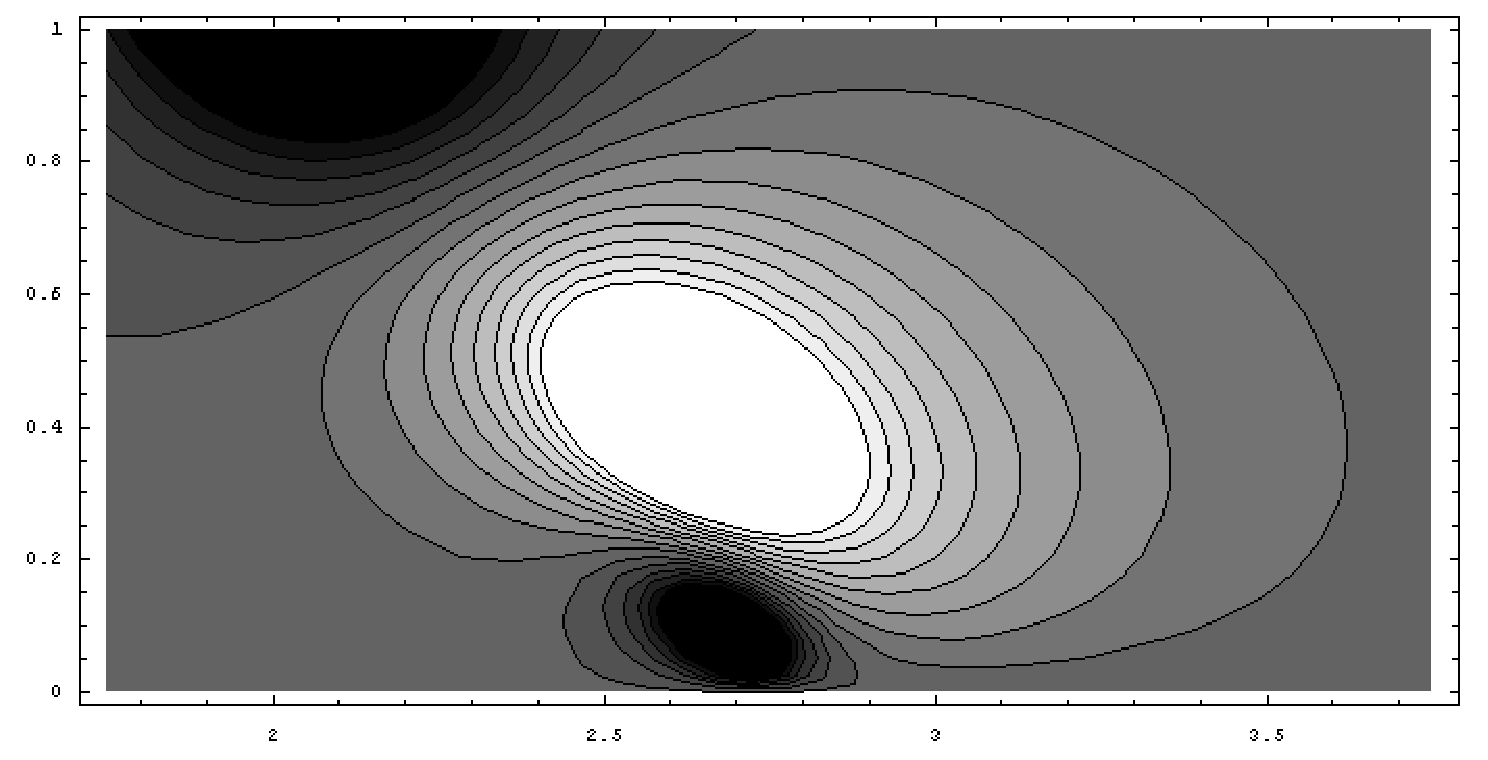
\includegraphics[width=4in]{img/sg_slope_n16_s05_2src_atop.eps}
\end{figure}
\end{center}

\end{slide}
%%%%%%%%%%%%%%%%%%%%%%%%%%%%%%%%%%%%%%%%%%%%%%%%%%%%%%%%%%%%%%%%%%%%%%%%%%%%%%%%
\begin{slide}

\begin{center}
Upper-Level Jet Streak Exit Region Ahead of a Surface Frontal Zone
\begin{figure}
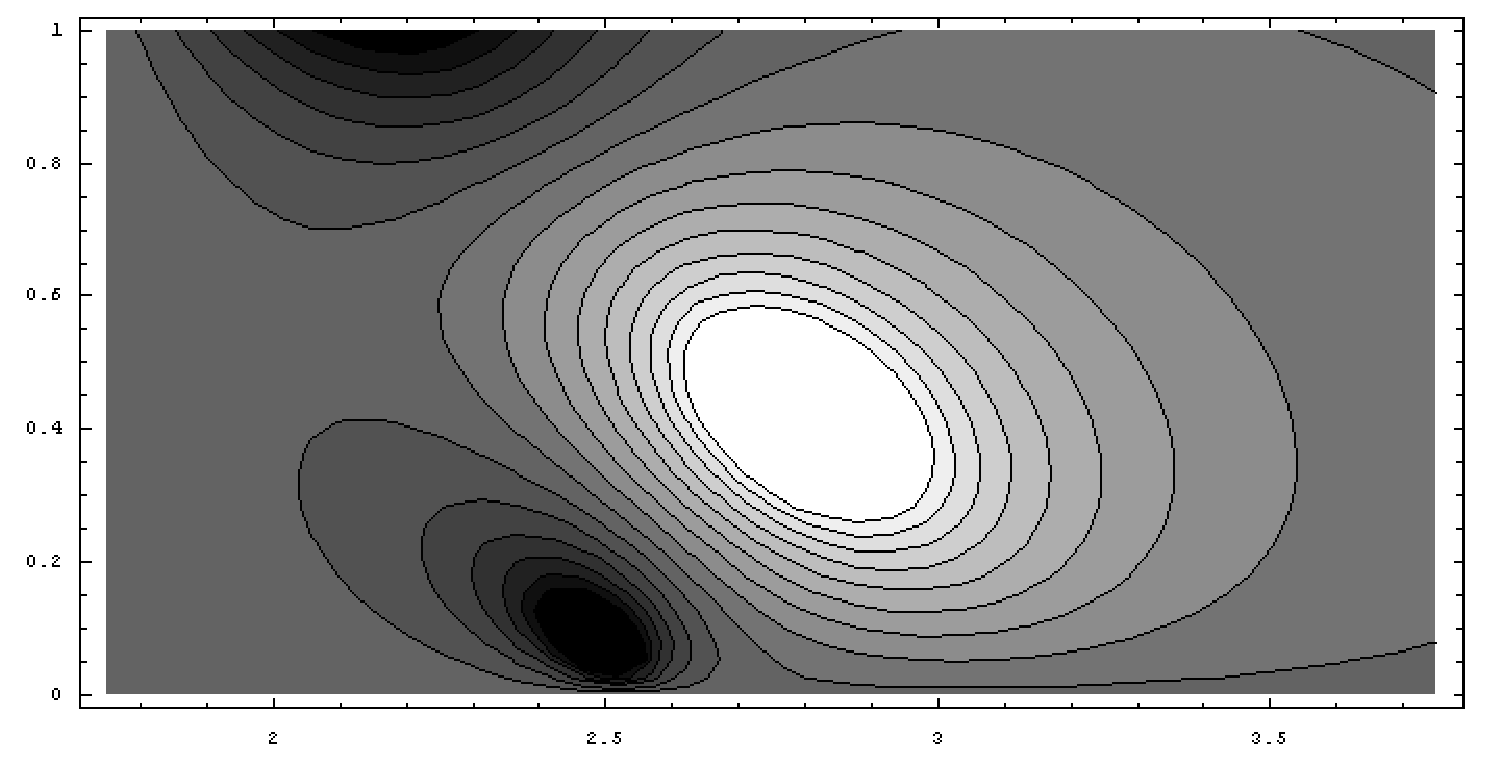
\includegraphics[width=4in]{img/sg_slope_n16_s05_2src_jetds.eps}
\end{figure}
\end{center}

\end{slide}
%%%%%%%%%%%%%%%%%%%%%%%%%%%%%%%%%%%%%%%%%%%%%%%%%%%%%%%%%%%%%%%%%%%%%%%%%%%%%%%%
\begin{slide}

\begin{center}
Upper-Level Jet Streak Entrance Region Behind a Surface Frontal Zone
\begin{figure}
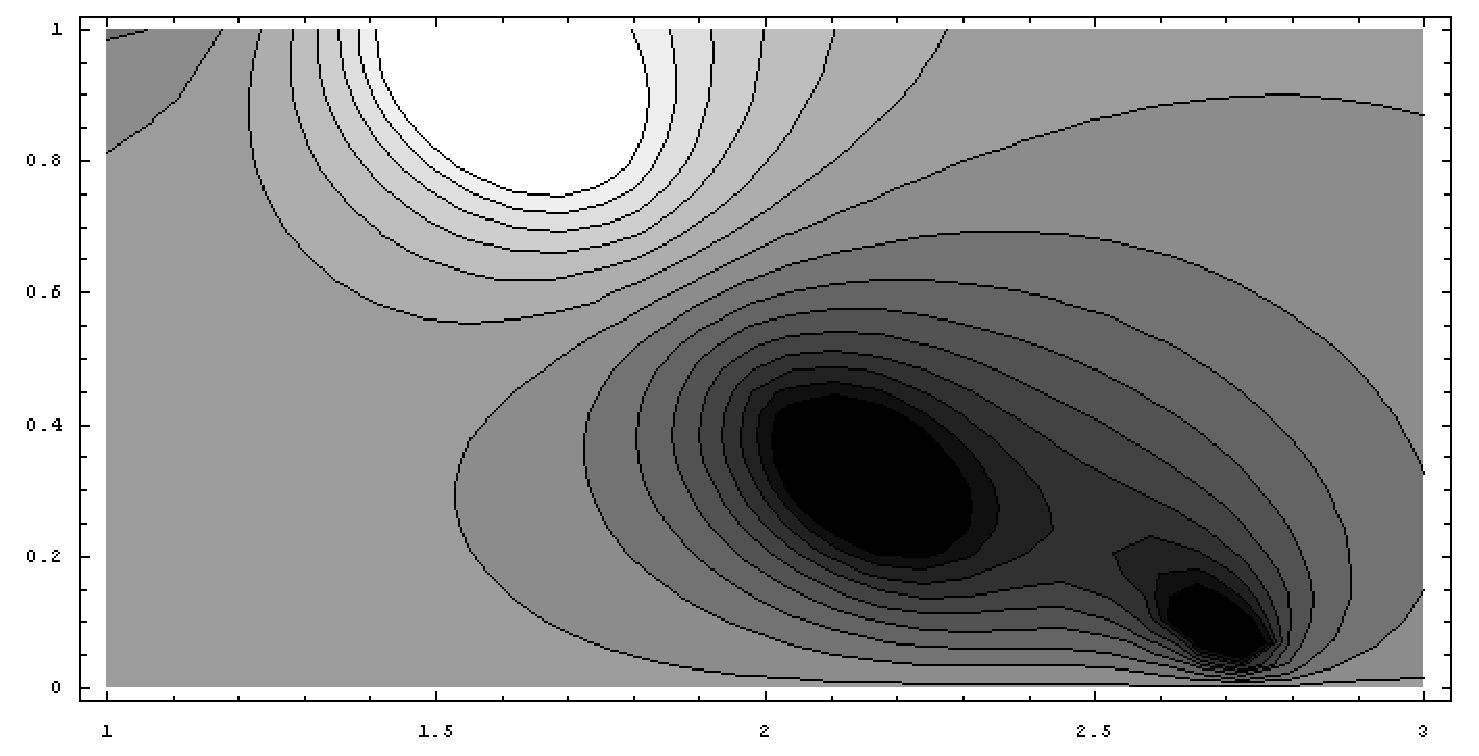
\includegraphics[width=4in]{img/sg_slope_n16_s05_entrjet.eps}
\end{figure}
\end{center}

\end{slide}
%%%%%%%%%%%%%%%%%%%%%%%%%%%%%%%%%%%%%%%%%%%%%%%%%%%%%%%%%%%%%%%%%%%%%%%%%%%%%%%%
\begin{slide}

\begin{center}
Horizontally Coupled Jet Streak Circulation
\begin{figure}
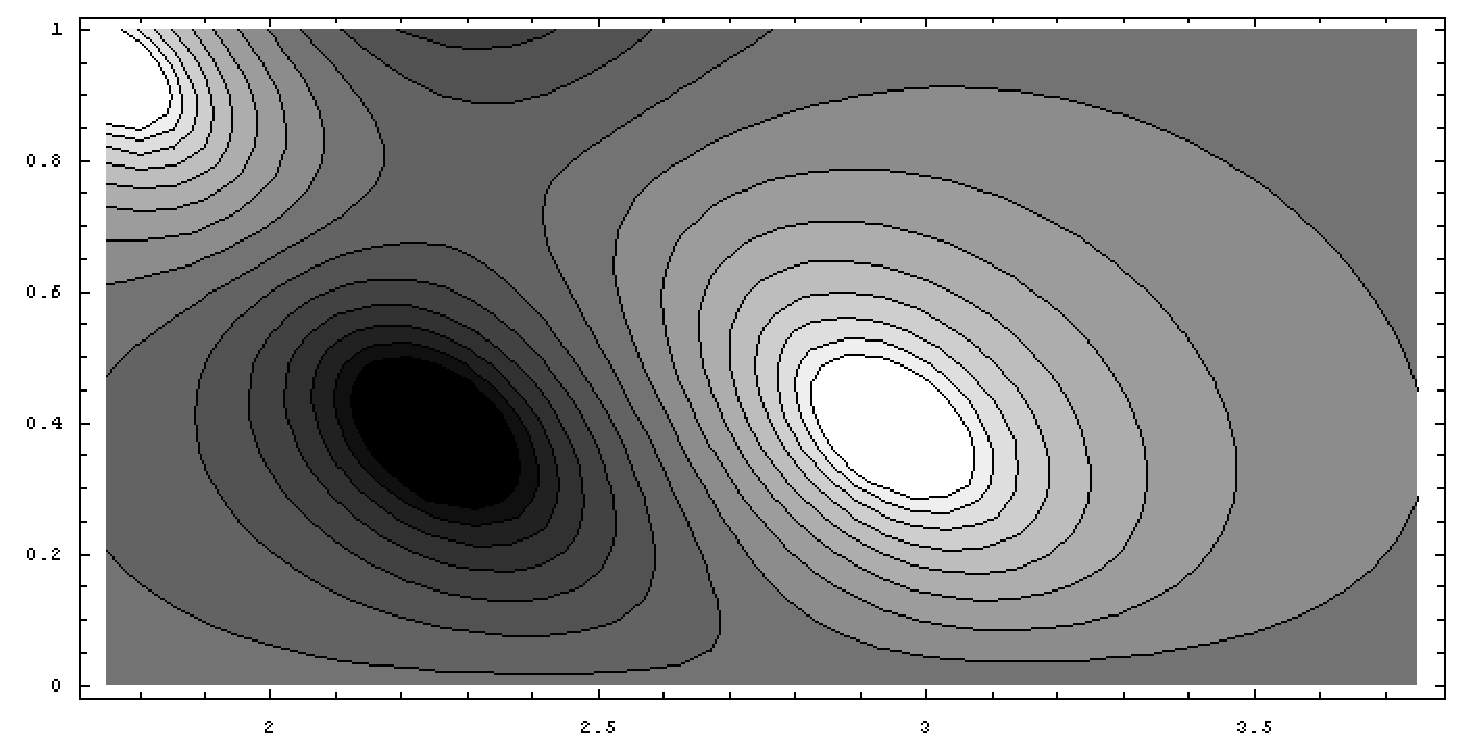
\includegraphics[width=4in]{img/sg_slope_n16_s05_2topjet.eps}
\end{figure}
\end{center}

\end{slide}
%%%%%%%%%%%%%%%%%%%%%%%%%%%%%%%%%%%%%%%%%%%%%%%%%%%%%%%%%%%%%%%%%%%%%%%%%%%%%%%%
\begin{slide}

\begin{center}
{\color{darkblue} \large QG Flows with Circular Curvature}

Jet Streak Exit Region Over Frontal Zone
\begin{figure}
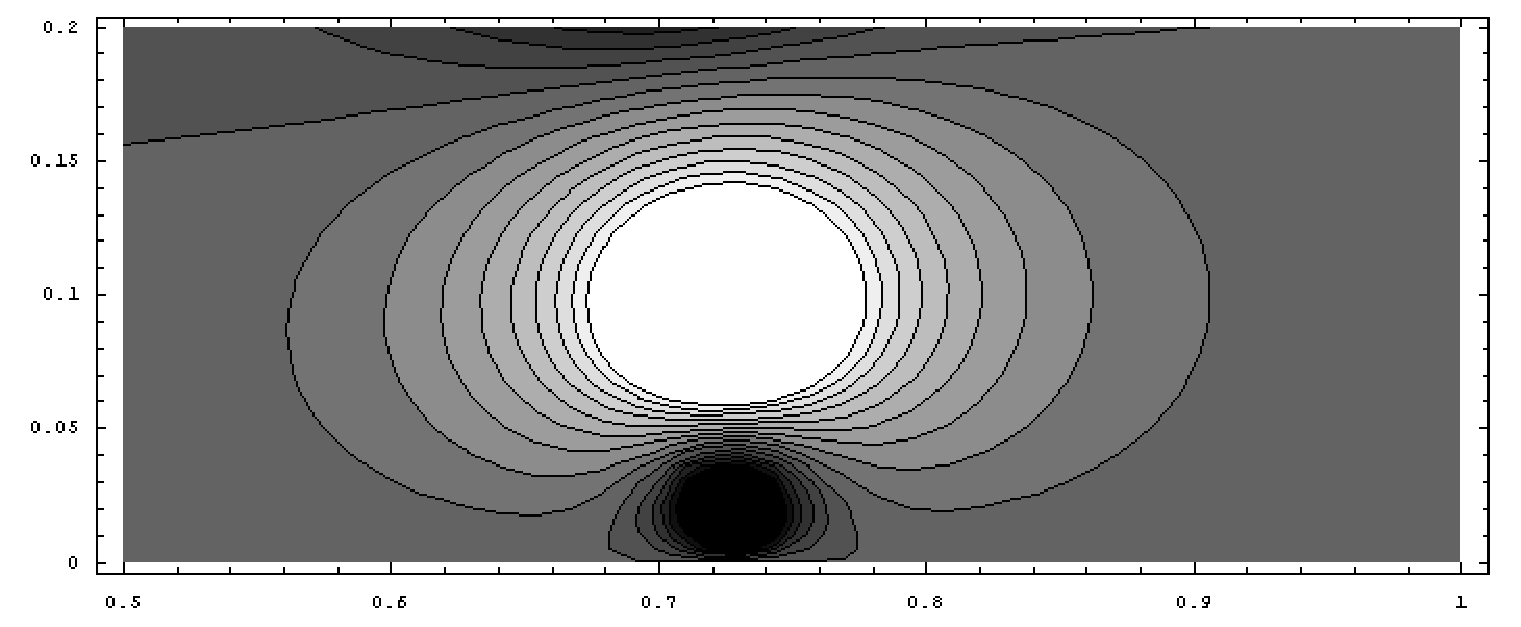
\includegraphics[width=3.2in]{img/qg_curve_n16_2src_atop.eps}
\end{figure}
Horizontally Coupled Jet Streak
\begin{figure}
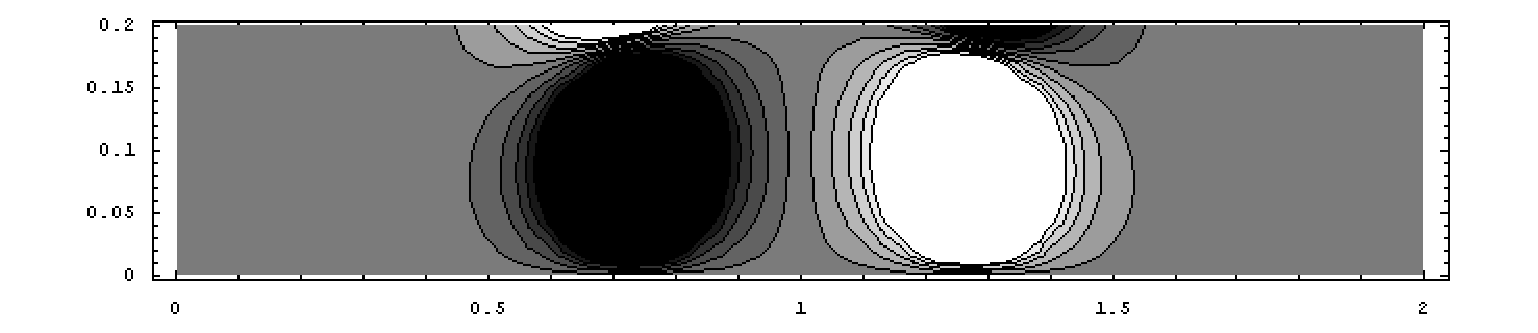
\includegraphics[width=3.5in]{img/qg_curve_n16_2topjet.eps}
\end{figure}
\end{center}

\end{slide}
%%%%%%%%%%%%%%%%%%%%%%%%%%%%%%%%%%%%%%%%%%%%%%%%%%%%%%%%%%%%%%%%%%%%%%%%%%%%%%%%
\begin{slide}

\begin{center}
{\color{darkblue} \large Concluding Remarks \\ \rule[0.15in]{\textwidth}{.03in}}
\end{center}

\begin{itemize}
\item Analytic structure of flow can be determined for simple variations in tropopause height

\item Slope (first order) and curvature (second order) effects were successfully solved; higher order curvature effects may have analytic solutions as well

\item These methods can also apply to variations in topography
\end{itemize}

\end{slide}
%%%%%%%%%%%%%%%%%%%%%%%%%%%%%%%%%%%%%%%%%%%%%%%%%%%%%%%%%%%%%%%%%%%%%%%%%%%%%%%%
\begin{slide}

\begin{center}
{\color{darkblue} \large Applications and Future Work}
\end{center}

\begin{itemize}
\item Potential to produce improved accuracy in vertical frontal flows without appealing to numerical PDE solutions

\item Frontogenesis on particular topographics, e.g. sloping valleys, may be applicable

\item Topographic or tropopause variations may generate Rossby waves - such an effect could lead to energy dissipation and frontolytic effects. Their role should be ascertained
\end{itemize}

\end{slide}
%%%%%%%%%%%%%%%%%%%%%%%%%%%%%%%%%%%%%%%%%%%%%%%%%%%%%%%%%%%%%%%%%%%%%%%%%%%%%%%%

\end{document}